% ------------------------------------------------------------------------ %
% !TEX encoding = UTF-8 Unicode
% !TEX TS-program = pdflatex
% !TEX root = ../Tesi.tex
% !TEX spellcheck = it-IT
% ------------------------------------------------------------------------ %
%
% ------------------------------------------------------------------------ %
% 	NOME CAPITOLO
% ------------------------------------------------------------------------ %
%
\chapter{Blockchain}
%
\label{cap:blockchain}
%
\section{Introduzione}
Una blockchain è una base di dati distribuita organizzata in blocchi, ciascuno dei quali contiene un insieme di record. Questi ultimi rappresentano la registrazione di un particolare evento associato ad un istante temporale (un timestamp). La struttura complessiva della rete assume la forma di una catena poichè ciascun blocco è legato al precedente, come è illustrato nella seguente immagine:
\begin{center}%
	\begin{figure}[h!]
		%
		\centering
		%
		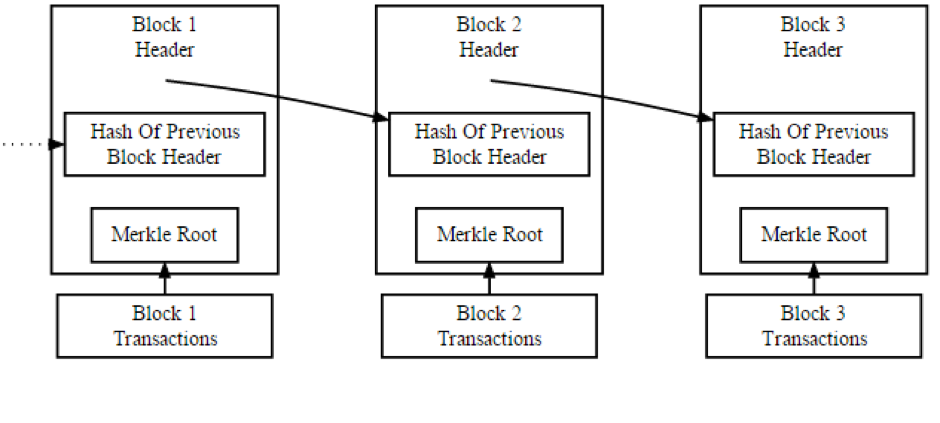
\includegraphics[width=.95\textwidth]{Blockchain/bloccoBlockchain}
		%
		\caption{Catena di blocchi in una blockchain}
		%
		\label{fig:catena di blocchi in una blockchain}
		%
	\end{figure}%
\end{center}
Il legame tra un blocco ed il suo predecessore viene realizzato attraverso l'inserimento, in ciascun blocco, di un riferimento al blocco precedente. Questa dipendenza all'indietro trova la sua conclusione nel blocco iniziale della catena, che solitamente viene generata da zero. Questa tecnologia nasce come infrastruttura della criptovaluta conosciuta come \emph{Bitcoin}, il cui fondatore, noto con lo pseudonimo di Satoshi Nakamoto, l'ha creata nel 2009 generando il primo blocco dopo aver spiegato il funziomento del sistema nel suo documento pubblicato un anno prima. \cite{bitcoin} \\
Ma questa non è l'unica definizione che si può dare della blockchain in quanto ogni definizione può mettere  in evidenza uno o più aspetti salienti della tecnologia stessa.
%
\paragraph{Blockchain come evoluzione del concetto di \enquote*{Ledger}} 
Con \emph{Ledger} si intende il \enquote*{libro mastro} in cui vengono registrate tutte le transazioni del sistema. Sotto quest'ottica la Blockchain è la realizzazione del \emph{Distributed Ledger}, come evoluzione dal \emph{Centralized Ledger}, passando per il \emph{Decentralized Ledger}. Tipicamente, la logica centralizzata è rappresentata dal tradizionale \enquote*{Centralized Ledger} con un rapporto rigorosamente centralizzato \enquote*{Uno-A-Tanti}, dove tutto deve essere gestito facendo riferimento a una struttura o autorità o sistema centralizzato. Nel Centralized Ledger la fiducia è nell’autorità, nell’autorevolezza del soggetto o sistema che rappresenta il \enquote*{centro} dell’organizzazione. \\
Dal modello centralizzato, si passa attraverso il \enquote*{Decentralized Ledger}, che ripropone la logica della centralizzazione a livello \enquote*{locale} con \enquote*{satelliti} organizzati a loro volta nella forma di Uno-A-Tanti che si relazionano a loro volta in una forma che ripete il modello Uno-A-Tanti. Non c’è più un \enquote*{grande} soggetto centrale ma ci sono tanti \enquote*{soggetti centrali}. La fiducia anche in questo caso viene delegata a un soggetto centrale, logicamente più vicino, ma comunque centralizzato. Le organizzazioni basate su Decentralized Ledger definiscono una Governance che stabilisce delle forme di coordinamento di tipo centralizzato. \\
Infine si arriva al \enquote*{Distributed Ledger}, ovvero ad una reale e completa logica distribuita dove non esiste più nessun centro e dove la logica di governance viene costruita attorno a un nuovo concetto di fiducia tra tutti i soggetti. Il processo decisionale passa attraverso un rigoroso processo di costruzione del Consenso.
%
\begin{center}%
	\begin{figure}[H]
		%
		\centering
		%
		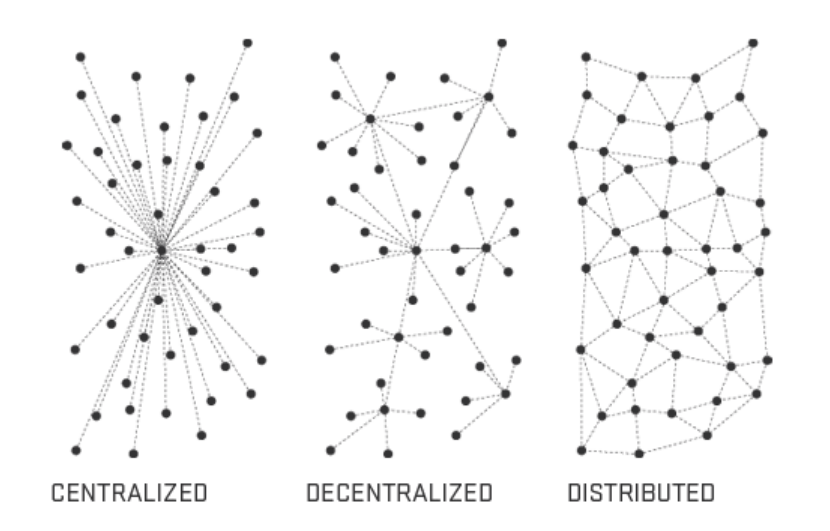
\includegraphics[height=5cm,width=.85\textwidth]{Blockchain/cdd}
		%
		\caption{Da Centralized a Decentralized Ledger}
		%
		\label{fig:da centralized a decentralized ledger}
		%
	\end{figure}%	
\end{center}
%
\section{Caratteristiche Generali}
%
La blockchain si evolve attraverso l'attività di un timestamp server distribuito, che prende un blocco di item e tramite la Marca Temporale\footnote{istante temporale o timestamping} marca il blocco e ne calcola l'hash. Mentre nei centralized ledger il punto di forza era localizzato nella fiducia che tutti i partecipanti dovevano avere nel gestore del central ledger (un soggetto di terze parti al di sopra dei partecipanti che garantisce la fiducia), nel distributed ledger la blockchain può essere considerata come una base di dati senza intermediari, ovvero che per utilizzarla non è necessario rivolgersi ad un server. Infatti le sue caratteristiche e la sua natura decentralizzata sono quelle che garantiscono l'affidabilità e la fiducia senza la presenza di un’autorità centrale che regoli le attività dei vari utenti. Questo ad esempio, nel caso di Bitcoin, si traduce nell'eliminazione di entità bancarie in grado di controllare (ed eventualmente anche alterare) le transazioni. \\
Una blockchain gode quindi delle seguenti proprietà:
\begin{enumerate}
	\item è distribuita: le informazioni sono replicate e dislocate su più nodi della rete;
	\item è inviolabile: essendo i blocchi condivisi tra più nodi ed dato che, per alterarne il contenuto è necessario il consenso della maggioranza assoluta, è improbabile che un attacco vada a buon fine;
	\item può essere pubblica (Unpermissioned Ledger) dove chiunque può controllare l'attività di chiunque, ma può anche essere privata (Permissioned Ledger) dove i partecipanti alla blockchain sono un numero limitato di attori che sono definiti come trusted. Le \gls{permissioned} sono più vicine alle esigenze di imprese ed istituzioni che vogliono comunque servirsi della tecnologia della blockchain;
	\item rispetta i requisiti di:
	      \begin{itemize}
	      	\item \emph{confidenzialità}: le informazioni sono accessibili solo agli utenti autorizzati;
	      	\item \emph{integrità}: ognuno può alterare solo i dati per cui è autorizzato;
	      	\item \emph{non ripudio}: le transazioni irrevocabili (caratteristica fondamentale della blockchain);
	      	\item \emph{autenticità}: vengono utilizzati meccanismi di cifratura per garantire l'autenticità nella blockchain.
	      \end{itemize}%
\end{enumerate}
%
\section{Architettura}
%
L'architettura di una blockchain (semplificata), può essere osservata nella seguente figura:
% \begin{center}
\begin{figure}[H]
	%
	\centering
	%
	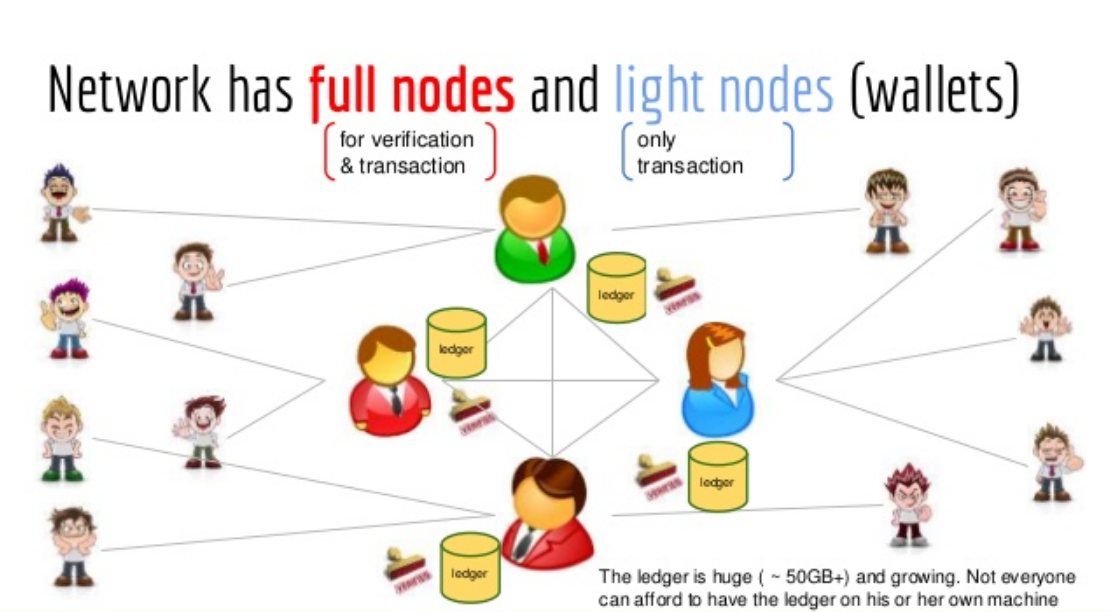
\includegraphics[width=.9\textwidth]{Blockchain/node}
	%
	\caption{Architettura di una blockchain su cui operano full node e lightweight node}
	%
	\label{fig:architettura di una blockchain}
	%
\end{figure}
%	
% \end{center}
Possiamo notare come l'assenza di intermediari si rispecchi a livello architetturale. Infatti la rete su cui si basa questa tecnologia è di tipo "peer to peer". Questa architettura risulta essere scalabile, dato che ciascun nodo può essere rimosso dalla rete o aggiunto alla stessa senza che l'attività complessiva risulti compromessa. Un nodo, per unirsi alla blockchain, ha due possibilità:
\begin{enumerate}
	\item diventare un \emph{full node}: il nodo deve scaricare una copia della blockchain al fine di poter effettuare operazioni e, al tempo stesso, validare le operazioni effettuate dagli altri utenti della blockchain;
	\item diventare un \emph{lightweight node}: il nodo può comunque partecipare alle attività della blockchain, senza però validare le operazioni degli altri utenti. Il vantaggio di un lightweight node risiede nel fatto che non deve scaricare l'intera copia della blockchain (ne scarica solamente una parte) per poter compiere delle operazioni ma agisce interrogando esso stesso uno dei full node presenti nella rete.
\end{enumerate}
%
\section{Mining e Proof of Work}
Il processo di consenso decentralizzato del Bitcoin richiede l'esistenza dei nodi nel network che continuamente tentano di produrre pacchetti di transazioni chiamati \enquote*{blocchi}. Il network produce all'incirca un blocco ogni dieci minuti ed ogni blocco contiene, come abbiamo detto in precedenza, una marca temporale, un numero casuale(nonce), un riferimento al precedente blocco (l'hash del precedente blocco) e una lista di tutte le transazioni che sono avvenute dal precedente blocco. Con il passare del tempo si crea quindi una persistente, sempre crescente catena che si aggiorna costantemente per rappresentare l'ultimo stato del libro mastro di Bitcoin. \\ 
Questo processo di creazione di un nuovo blocco va sotto il nome di \emph{mining} e viene realizzato da entità facenti parte della rete chiamate \emph{miners}. Per generare un blocco generalmente è necessario:
\begin{itemize}
	\item stabilire quali transazioni andranno a far parte del nuovo blocco;
	\item verificare la validità di queste transazioni;
	\item selezionare il blocco più recente della blockchain (l'ultimo creato) ed inserire il suo hash nel nuovo blocco;
	\item risolvere infine la \emph{Proof-of-work} (POW) e, contemporaneamente, assicurarsi che eventuali blocchi generati prima del proprio siano validi.
\end{itemize}
La componente principale dell'attività di mining è la fase che riguarda la Proof-of-work, ovvero quella che involve tutti i miners e che li vede impegnati nella risoluzione di un problema ad elevata complessità (in cui è richiesta un'elevata capacità di calcolo), la cui risoluzione avrà come risultato l'aggiunta di un nuovo blocco alla rete e un pagamento in Bitcoin al miner che ha risolto il blocco. La POW si articola nel seguente modo: viene utilizzato l'algoritmo di hash SHA-256 che produce un numero formato da 256 bit. L'oggetto su cui si applica la funzione di hash, costituito dal blocco di transazioni corrente, è il cosiddetto \emph{header}\footnote{comprende il numero di versione del protocollo, l’hash del blocco precedente, l’hash di un sommario delle transazioni del blocco corrente, una timestamp (cioè data e ora di creazione del blocco) e il grado di difficoltà stabilito per il blocco corrente blocco e il nonce} del blocco. L'obiettivo di questa sfida è ottenere un valore di hash inferiore di un target regolato dinamicamente\footnote{generalmente il target viene ricalibrato dal network ogni 2016 blocchi, al fine di lasciar costante il tempo di produzione di un blocco (10 minuti)}. Poichè SHA-256 è progettato peressere una funzione completamente imprevedibile e pseudo-randomica, l'unico modo per creare un blocco valido è un insieme di tentativi con l'incremento ripetuto del nonce al fine di trovare il valore richiesto dalla proof-of-work. Si nota come questa sfida computazionale sia difficile da completare ma facilmente verificabile all'interno della rete. \\
Una volta risolta la proof-of-work e generato il blocco associato, per alterare una transazione in un blocco, bisognerebbe modificare anche tutte le transazioni passate (essendo esse collegate in cascata da una serie di firme digitali) e rimettere quindi in gioco tutta la capacità di calcolo utilizzata nella risoluzione perchè si dovrebbe rimodificare quel blocco e tutti i suoi successori. Infine al minatore che ha risolto il blocco generato viene ricompensato con una certa quantità di bitcoin. In altre implementazioni della blockchain esistono altri strumenti per stabilire chi andrà a minare il blocco successivo:
\begin{itemize}
	\item \emph{proof-of-stake}: il diritti di minare viene concesso in funzione della quantità di denaro che si possiede (adatta in contesti con bassa capacità di calcolo);
	\item \emph{prrof-of-burn}: il miner può  aggiudicarsi la contesa dimostrando di aver consumato monete, inviandole ad un indirizzo non suo e non potendole quindi più utilizzare, dimostrando di aver fatto un sacrificio.
\end{itemize}
%
\section{Le transazioni}
%
Una transazione rappresenta un trasferimento di valore che viene registrato in un blocco della blockchain. Bitcoin, ad esempio, utilizza un sistema di transizioni di stato dove:
\begin{itemize}
	\item stato: consistente nella proprietà dello status di tutti i bitcoins esistenti;
	\item funzione di transizione di stato: riceve uno stato ed una transizione e trasmette un nuovo stato che ne costituisce il risultato.
\end{itemize}
In bitcoin lo \enquote*{stato} è la raccolta di tutte le monete (tecnicamente definite come \enquote*{transazioni in uscita non spese} o UTXO\footnote{Unspend Transaction Output}). Ogni UTXO ha una denominazione ed un proprietario definito da un indirizzo di 20 byte che corrisponde essenzialmente alla sua chiave pubblica. Una transazione viene costruita in riferimento a transazioni passate da cui prelevare i fondi che vengono trasferiti al nuovo destinatario. Quindi ogni transazione contiene:
\begin{itemize}
	\item uno o più vettori di input, dove ogni input contiene un riferimento ad uno UTXO esistente ed una firma crittografica prodotta da una chiave privata associata all'indirizzo del proprietario\footnote{in questo modo si evita la possibilità che una persona spenda monete non di sua proprietà};
	\item uno o più vettori di output, dove ogni output contiene un nuovo UTXO che deve essere aggiunto allo stato;
\end{itemize}
Una transazione può avvenire nel seguente modo:
\begin{center}
	\begin{figure}[H]
		%
		\centering
		%
		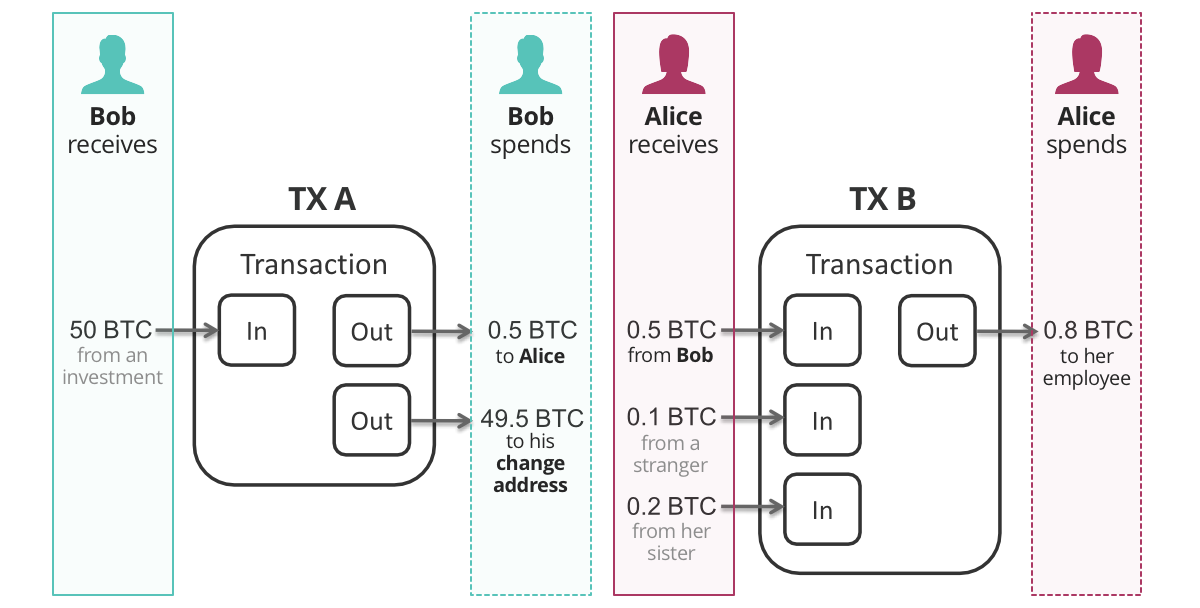
\includegraphics[width=.9\textwidth]{Blockchain/bitcoinTransaction}
		%
		\caption{Esempio di transazione}
		%
		\label{fig:esempio di transazione}
		%
	\end{figure}
\end{center}
%
Ogni transazione effettuata viene quindi inviata a tutti i nodi i quali raccolgono le nuove transazioni in un blocco e partecipano alla proof-of-work per minare il nuovo blocco. Un blocco, per essere accettato deve contenere al suo interno solamente transazioni valide e non deve essere presente il problema del \emph{double spending} (spendere gli stessi soldi due volte).
%
\section{Permissioned Blockchain}
%
Sono attualmente presenti numerosi progetti di blockchain permissioned, come il progetto Hyperledger\cite{website:hyperledger} della Linux Foundation, o la rete Gem Health\cite{gem}. Alcuni ritengono che le blockchain private siano sono un modo alternativo di definire uno shared-database. Infatti, come sostenuto da Gideon Greenspan, CEO di CoinSciences :"se fiducia e robustezza non sono un target, non c'è nulla che una blockchain possa fare ed un database no", a conferma del fatto che le due tecnologie sono tutto sommato alternative, ma non analoghe.\\
Nel presente lavoro di tesi, verrà utilizzata una blockchain \emph{permissioned} (privata). Una blockchain permissioned gode innanzitutto delle stesse proprietà di una blockchain pubblica, ovvero:
\begin{itemize}
	\item è una rete peer-to-peer decentralizzata dove ogni partecipante mantiene una replica di un libro mastro di transazioni firmate digitalmente;
	\item le repliche sono mantenute sincronizzate attraverso un protocollo di consenso;
	\item sono presenti garanzie di immutabilità anche in presenza di partecipanti maligni.
\end{itemize}
Quello che una blockchain permissioned aggiunge ad una blockchain pubblica è un meccanismo di controllo degli accessi integrato nei client, così che i peer possano essere aggiunti nella rete sulla base di un valore di controllo (un certificato o un indirizzo ad esempio). La scelta di utilizzare blockchain permissioned si adatta alla volontà di aziende, governance e pubbliche amministrazioni che vogliono utilizzare il livello tecnlogico e la sicurezza raggiunte dalle blockchain, mantenendo al tempo stesso la loro presenza all'interno della rete, necessaria per mantenere il controllo sui partecipanti. Queste blockchain sono sì adatte a gestire moneta, ma le loro potenzialità si manifestano soprattutto in altri campi come la condivisione di dati medicali (i quali non devono essere alterati in alcun modo) o la catena di distribuzione di farmaci (per evitare frodi a qualsiasi livello della supply-chain, dalla produzione alla vendita al dettaglio). \\
Le blockchain permissioned imitano il processo di sicurezza utilizzato dalle blockchain pubbliche come Bitcoin, ma essendo il numero e l'identità dei partecipanti conosciuto, non c'è il bisogno della proof-of-work o della proof-of-stake, mentre utilizzano la stessa crittografia e le stesse strutture dati come i Merkle trees\cite{merkle} per assicurare che transazioni non valide non siano aggiunte alla blockchain. I meccanismi di consenso più popolari includono Raft\cite{raft} e Juno\cite{juno}. Questi protocolli di consenso funzionano sulla base di un modello leader-follower, in cui per ogni blocco viene selezionato un leader che crea il blocco e lo aggiunge alla blockchain, mentre errori ed anomalie vengono automaticamente corretti dal sistema. \\
Anche le blockchain permissioned godono della robustezza tipica della loro controparte pubblica dato che mantengono la proprietà di essere ridondanti e quindi estremamente fault-tolerant. Ogni nodo processa le transazioni, perciò nessun nodo risulta indispensabile. Per questo motivo, e per la natura peer-to-peer della rete, la replicazione che nei database viene realizzata tramite tecniche apposite, nelle blockchain è un processo naturale dato che i nodi si sincronizzano a vicenda. Infine ogni volta che si effettua una transazione rispetto ai database tradizionali, i sistemi basati su blockchain devono farsi carico di ulteriori oneri:
\begin{itemize}
	\item verifica della firma: ogni transazione deve essere firmata con uno schema di crittografia a chiave pubblica;
	\item meccanismo di conenso: i nodi della rete devono raggiungere il consenso;
	\item ridondanza delle operazioni.
\end{itemize}
Questo ovviamente si traduce in prestazioni minori rispetto ai database tradizionali.\\
Le blockchain permissioned quindi cercano di unire le capacità di prestazione e riservatezza (tipiche dei database tradizionali) con i meccanismi di fault-tolerance e disintermediazione (per quanto possibile nelle blockchain private) tipiche della blockchain.
%
\section{Limiti delle Blockchain}
%
Per quanto valida la tecnologia della blockchain come quella presentata ed implementata da Bitcoin, essa presenta dei limiti nel caso in cui si voglia costruire applicazioni avanzate su di essa. Infatti Bitcoin presenta un linguaggio di scripting estremamente limitato, che soffre dei seguenti limiti:
\begin{enumerate}
	\item \emph{mancanza di completezza del linguaggio di Turing}: ovvero, mentre esiste un grande sottoinsieme di calcolo che il linguaggio di scripting del Bitcoin supporta, quest ultimo non supporta tutto. Infatti troviamo la mancanza dei \enquote{loop};
	\item \emph{cecità del valore}: non c'è un modo per un UTXO di fornire un controllo a setaccio sull'ammontare ritirabile;
	\item \emph{mancanza di stato}: UTXO può essere sia speso che non speso, non c'è possibilità per scripts di mantenere altri stati interni oltre questo.
\end{enumerate}
La soluzione sta nelle blockchain di seconda generazione che riprendono un concetto teorizzato negli anni '70, gli Smart Contract, e lo implementano all'interno della loro rete peer-to-peer.
%
